\section{ROS file system}

The foundation of the ROS file system revolves around packages, depicted in the diagram below. 
\begin{figure}[H]
    \centering
    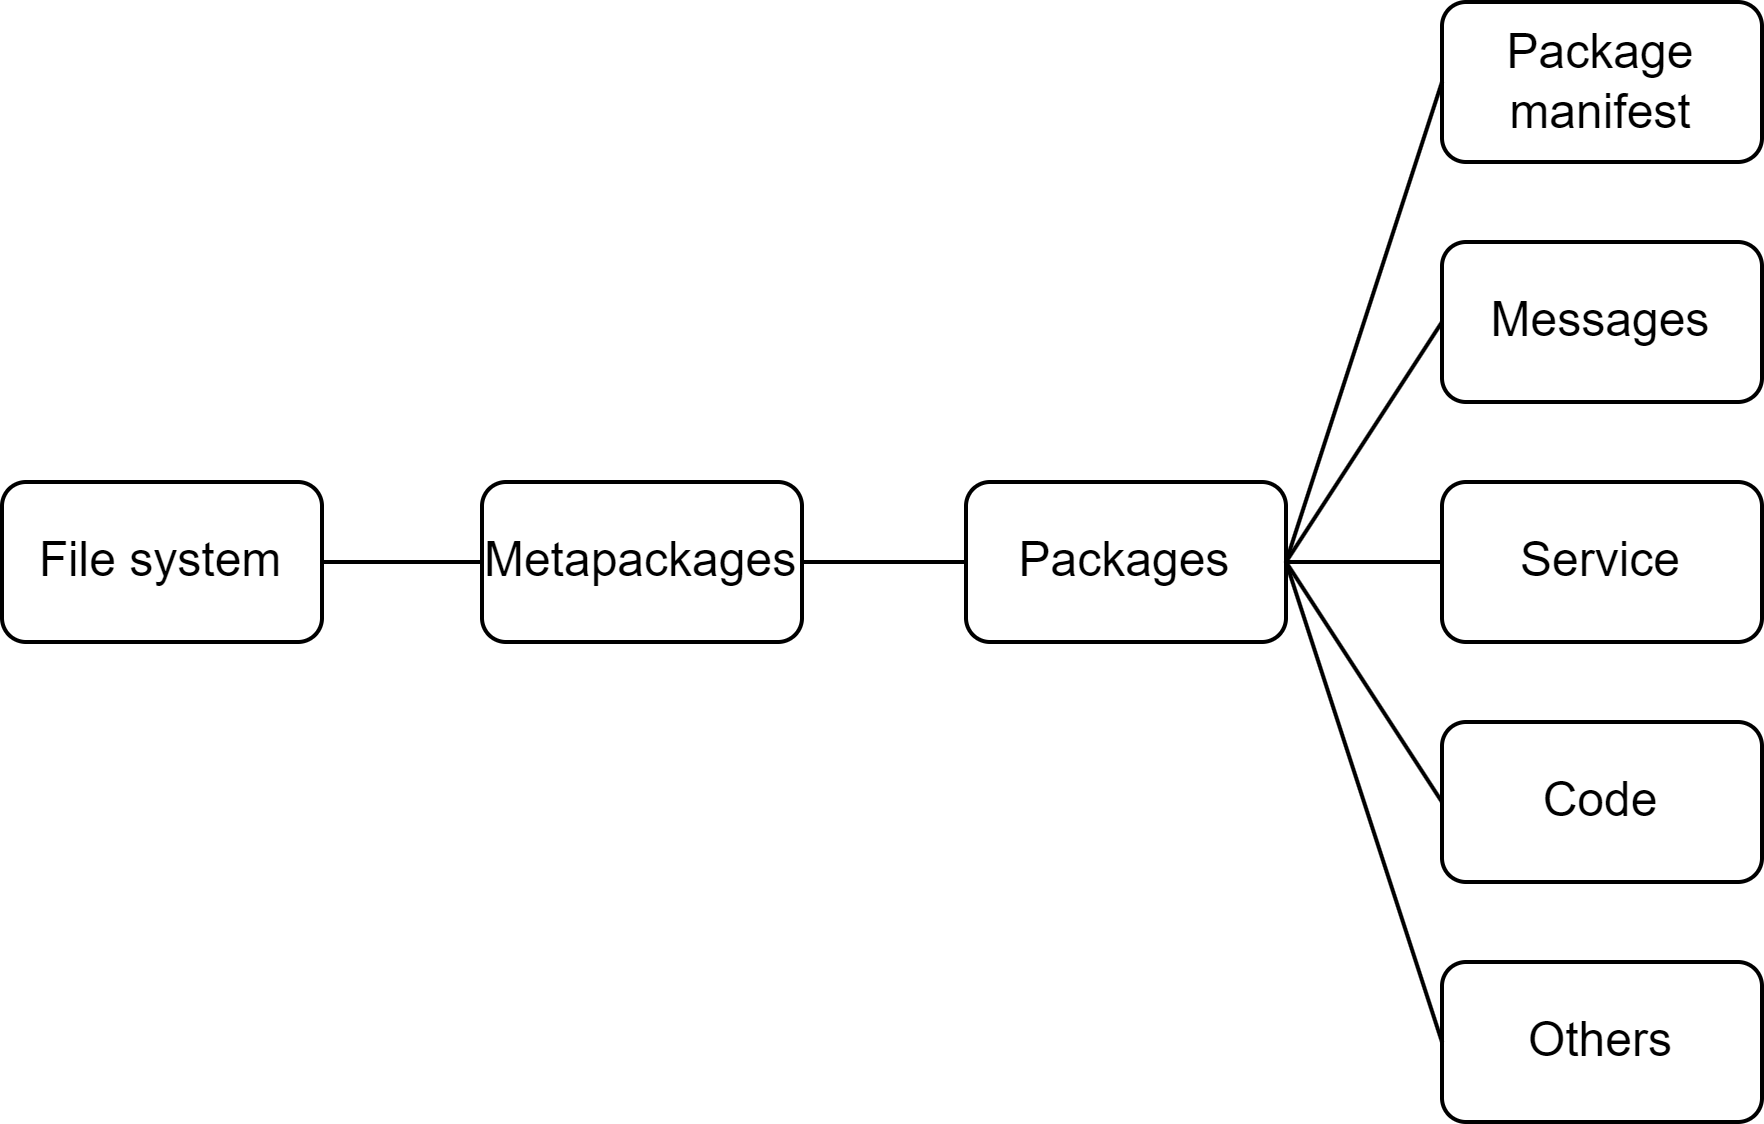
\includegraphics[width=0.75\linewidth]{images/fs.png}
    \caption{ROS file system}
\end{figure}
Packages serve as the fundamental units within the ROS file system. 
They are essential references for most ROS commands and encompass nodes, messages, and services. 
Each package is described by a \texttt{package.xml} file and acts as a mandatory container for its contents.

Additionally, there are metapackages, which aggregate logically related elements. 
Unlike packages, metapackages are not directly utilized when navigating the ROS file system. 
They contain other packages and are described by a package.xml file as well, but they are not obligatory components.